\documentclass[11pt,a4paper]{article}
\usepackage{fontspec}
\setmainfont{NotoSerifCJKkr-Regular.otf}[Path=fonts/,BoldFont=NotoSerifCJKkr-Bold.otf,ItalicFont=NotoSerifCJKkr-Regular.otf]
\setsansfont{NotoSerifCJKkr-Regular.otf}[Path=fonts/,BoldFont=NotoSerifCJKkr-Bold.otf]
\setmonofont{DejaVu Sans Mono}[Scale=0.79]
\XeTeXlinebreaklocale "ko"
\XeTeXlinebreakskip=0pt plus 1pt
\usepackage[margin=23mm,top=23mm,bottom=23mm,headheight=15pt]{geometry}
\usepackage{amsmath,amssymb,amsthm,mathtools,mathrsfs}
\usepackage{booktabs,tabularx,longtable,array,graphicx,float}
\usepackage[dvipsnames]{xcolor}
\usepackage{enumitem,caption,fancyhdr,titlesec}
\usepackage{tikz}
\usetikzlibrary{arrows.meta,positioning,calc}
\usepackage{hyperref}
\providecommand{\tightlist}{\setlength{\itemsep}{0pt}\setlength{\parskip}{0pt}}
\newcommand{\passthrough}[1]{#1}
\hypersetup{unicode=true,colorlinks=true,linkcolor=MidnightBlue,urlcolor=MidnightBlue,citecolor=MidnightBlue,pdftitle={WU088 HH PHYS18: HH와 birth의 혼합 응답과 유한 상호작용},pdfauthor={WU088 HH 연구}}
\urlstyle{same}
\setlength{\emergencystretch}{3em}
\setlength{\parskip}{0.34em}
\setlength{\parindent}{1em}
\widowpenalty=10000\clubpenalty=10000
\linespread{1.10}
\setlist{itemsep=0.18em,topsep=0.35em,leftmargin=1.6em}
\captionsetup{font=small,labelfont=bf}
\renewcommand{\figurename}{그림}
\renewcommand{\tablename}{표}
\renewcommand{\contentsname}{목차}
\renewcommand{\refname}{참고 문헌과 원자료}
\renewcommand{\proofname}{증명}
\titleformat{\section}{\large\sffamily\bfseries\color{MidnightBlue}}{\thesection}{0.7em}{}
\titleformat{\subsection}{\sffamily\bfseries}{\thesubsection}{0.7em}{}
\pagestyle{fancy}\fancyhf{}
\fancyhead[L]{\small\sffamily WU088\_HH / PHYS18 이론}
\fancyhead[R]{\small\sffamily 2026-10-13 KST}
\fancyfoot[C]{\thepage}
\newcommand{\dd}{\mathrm d}
\newcommand{\diag}{\operatorname{diag}}
\newcommand{\ex}{\operatorname{exact64}}
\newcommand{\BB}{\mathcal B}
\newcommand{\HF}{\mathcal H_F}
\newcommand{\R}{\mathsf R}
\newcommand{\RF}{\mathsf R_F}
\newcommand{\ew}{e_w}
\newcommand{\exx}{e_x}
\newcommand{\nS}[1]{\left\lVert#1\right\rVert_S}
\newcommand{\nI}[1]{\left\lVert#1\right\rVert_\infty}
\newcommand{\magv}{\operatorname{mag}}
\newtheorem{theorem}{정리}
\newtheorem{lemma}{보조정리}
\newtheorem{proposition}{명제}
\theoremstyle{definition}\newtheorem{definition}{정의}

\begin{document}
\begin{titlepage}
\centering
\vspace*{16mm}
{\Large\sffamily WU088\_HH / PHYS18 이론 연구 보고서\par}
\vspace{9mm}
{\huge\sffamily\bfseries HH와 birth의 혼합 응답\par}
\vspace{4mm}
{\LARGE\sffamily 상관된 endpoint 결함과 유한 상호작용\par}
\vspace{12mm}
{\large 같은 COMMON, 같은 전역 $\lambda,b$, 원 $C^2$ 물리계\par}
\vspace{10mm}
\begin{minipage}{0.88\textwidth}
\setlength{\parindent}{0pt}
두 half와 Full의 온도 차이를 $F=\Delta T=T_2-T_F$로 두었을 때,
원 signed 구간 입력으로 전체 매개변수 사각형에서 다음 포함을 얻었다.
\[
\boxed{F_{\lambda b}\in
[-2.668505746423,\,-2.118796636045]\times10^{-12}\ {\rm K}.}
\]
같은 구간은 네 모서리의 유한 상호작용
$\mathcal I=F(1,1)-F(1,0)-F(0,1)+F(0,0)$도 포함한다.
작은 1차 결함을 보존한 혼합 잔차, 35개 광자/guard 좌표의 mixed jet,
원 Full 역연산자와 유한 온도 분수를 결합한 결과다.
\end{minipage}
\vfill
{\large\sffamily 2026-10-13 KST\par}
\vspace{3mm}
{\small \texttt{physmath-research-loop} 내장 규약 1.0.0 / THEORY R1--R10\par}
\vspace{3mm}
{\small 선행 단위 PHYS17: \texttt{ba5f2693c5c1222b}\par}
\end{titlepage}
\setcounter{tocdepth}{2}
\tableofcontents
\clearpage
\section{결과와 연구 범위}

이번 PHYS18은 PHYS17에서 열린 HH--birth 혼합 응답을 실제로 계산한다.
PHYS16은 동일한 COMMON에서 시작한 두 half의 끝점 $g_2$와 Full의 끝점
$g_F$ 사이의 결함 $d=g_2-g_F$를 포함했고, PHYS17은
$d_\lambda,d_b$와 $F_\lambda<0$, $F_b>0$를 포함했다.
현재 질문은 birth를 바꿀 때 HH 방향의 온도 결함 응답이 얼마나 달라지는지,
또는 HH를 바꿀 때 birth 방향의 응답이 얼마나 달라지는지다.
두 질문의 공통 판별량은 $F_{\lambda b}$다.

\subsection{고정한 물리계와 입력}

매개변수는 동일한 전역 $\lambda,b\in[0,1]$이고, admissible $\alpha$를
고정한 원 source-aligned geometric-isotropic $C^2$ 계열을 사용한다.
기체 상태는 $g=(x_{\rm HII},y_{\rm HeII},y_{\rm HeIII},w)$이며
$w$의 단위는 ${\rm eV/H}$다. 광자 33개 군과 number/energy guard 두
좌표를 합친 35개 광자 좌표를 같은 연산 그래프에 유지한다.
두 half의 길이는 각각 $h=625000000\ {\rm s}$이고 Full의 길이는 $2h$다.
시각은 $t_0=160000000000$, $t_1=160625000000$,
$t_2=161250000000\ {\rm s}$다.

원 $C,B,q,S$는 PHYS15에 보존된 Full 자료다.
$q=\operatorname{exact64}(0.00011736830563768177)<1$과
$S=\operatorname{exact64}(0.015,0.01,0.01,0.5)$를 그대로 사용한다.
여기서 \texttt{exact64}는 저장된 binary64 leaf의 정확한 유리수 값이다.
온도 상수는 $C_T=2\,\mathrm{eV}_{\rm erg}/(3k_B)$이고,
$f_2=\operatorname{exact}(n_{\rm He,stored})/\operatorname{exact}(n_H)$,
$\ell_e=(1,f_2,2f_2,0)$를 사용한다.
$\Pi_2=1+f_2+\ell_e g_2$, $\Pi_F=\Pi_2-\ell_e d>0$에서 유한 분수를
계산한다. 원 $C^2$ 구간, root hull, 전처리 역 포함의 전제를 재사용한다.
상속 계약의 입력 24개는 크기와 SHA-256이 모두 일치했다.

\subsection{실제 혼합 포함}

혼합 도함수 $W=\partial_{\lambda b}g_2$와
$W_d=\partial_{\lambda b}(g_2-g_F)$는 보통의 편미분이며 Taylor 계수로
나누지 않는다. 표~\ref{tab:mixed-gas}는 최종 교차 포함을 보인다.

\begin{table}[H]
\centering\small
\caption{최종 mixed gas defect 포함. 두 매개변수는 무차원이다.}
\label{tab:mixed-gas}
\begin{tabular}{lll}\toprule
좌표 & 구간 & 단위 \\\midrule
$W_{d,x_{\rm HII}}$ & $[3.428209698898\times10^{-17},\ 4.498894132315\times10^{-17}]$ & 1 \\
$W_{d,y_{\rm HeII}}$ & $[-2.296697834724\times10^{-22},\ 5.758083648551\times10^{-23}]$ & 1 \\
$W_{d,y_{\rm HeIII}}$ & $[-9.420366340430\times10^{-24},\ -2.612148448548\times10^{-24}]$ & 1 \\
$W_{d,w}$ & $[-4.336773175632\times10^{-16},\ -3.600882004347\times10^{-16}]$ & $\mathrm{eV/H}$ \\
\bottomrule\end{tabular}
\end{table}


같은 양의 분모와 Full 온도 covector로 전달하면
\begin{equation}
 F_{\lambda b}\in[L_M,U_M]
 =[-2.668505746423,-2.118796636045]\times10^{-12}\ {\rm K}.
 \label{eq:main-mixed}
\end{equation}
이 수치는 exact rational endpoint를 바깥쪽으로 반올림한 표시다.
보존된 기계 결과에는 전체 유리수 양 끝점이 들어 있다.
따라서 $F_{\lambda b}<0$의 margin은 적어도 $2.118796636045\times10^{-12}\ {\rm K}$다.
입력 계열의 전체 사각형을 포함하는 판정이며 표본점 차분을 사용하지 않는다.

\begin{figure}[H]
\centering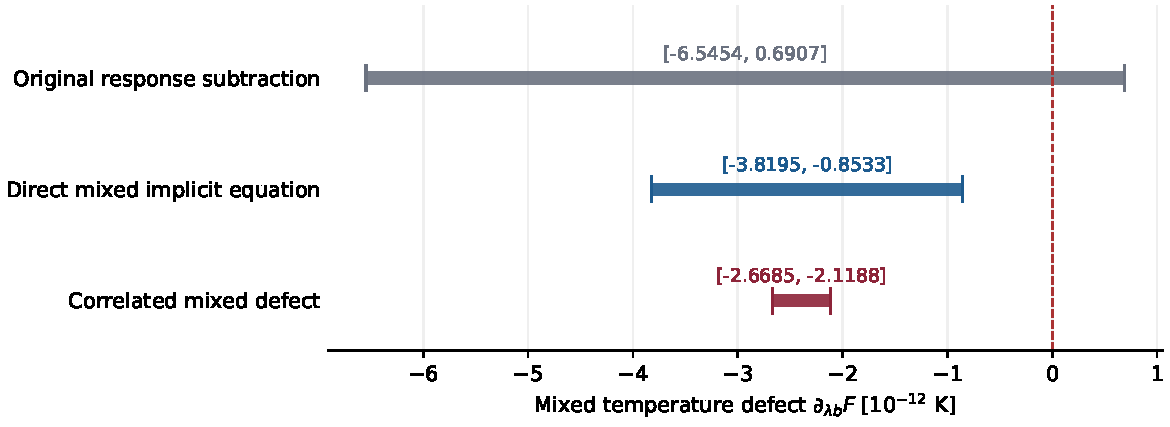
\includegraphics[width=0.97\linewidth]{figures/mixed_enclosure_comparison.pdf}
\caption{같은 유한 온도 분수에 전달한 세 가지 혼합 포함. 원 $W_2-W_F$
성분별 차는 0을 포함한다. 직접 암묵식은 음수를 판별하며, 작은 결함을
보존한 상관식은 가장 좁은 구간을 준다. 가로축은 $10^{-12}\ {\rm K}$다.}
\label{fig:comparison}
\end{figure}

\subsection{유한 매개변수 변화의 귀결}

$\lambda_1>\lambda_0$, $b_1>b_0$인 사각형에서 미적분학의 기본정리를
두 번 적용하면
\begin{align}
&F(\lambda_1,b_1)-F(\lambda_1,b_0)
-F(\lambda_0,b_1)+F(\lambda_0,b_0)\notag\\
&\qquad\in[L_M,U_M](\lambda_1-\lambda_0)(b_1-b_0)<0.
\label{eq:rectangle}
\end{align}
특히 단위 사각형의 $\mathcal I$도 식~\eqref{eq:main-mixed}의 구간에 들어간다.
이전 PHYS17의 $|\mathcal I|\le1.958485175177039\times10^{-9}\ {\rm K}$에
비해 현재 절댓값 상계는 약 734배 작고 부호도 결정된다.

$b$가 커지면 $F_\lambda$는 더 음수가 되고, $\lambda$가 커지면
양수인 $F_b$는 조금 줄어든다. 두 1차 방향의 부호는 PHYS17의 전역
구간에 의해 유지된다. 혼합 변화의 크기는 HH 1차 방향의 최소 절댓값에
대해 약 $0.033\%$ 이하, birth 1차 방향에 대해 약
$3.94\times10^{-6}\%$ 이하다.

축 위의 정확한 응답으로 만든 가법 표현
$F_{\rm sep}(\lambda,b)=F(\lambda,0)+F(0,b)-F(0,0)$에 대해서는
\begin{equation}
F(\lambda,b)-F_{\rm sep}(\lambda,b)
\in[L_M,U_M]\lambda b.
\label{eq:separable}
\end{equation}
따라서 이 가법 표현은 내부에서 실제 $F$보다 크며, 그 오차는 최대
$2.668506\times10^{-12}\lambda b\ {\rm K}$로 포함된다.
축 위 응답 자체를 새로 근사할 때의 오차는 그 근사 계약에 따로 포함한다.

\subsection{물리적 구성과 폭의 원인}

고정된 기체에서 원 $H_{\lambda b}=0$이다. 실제 혼합 응답은 기체의
암묵적 변화, 광자 흡수의 상태 의존성, 유한 온도의 입자수 분모에서 생긴다.
같은 $J_F^{-1}$와 같은 온도 covector로 각 강제항을 전달하여 이 연결을
분리했다. 가장 큰 음의 항 두 개는 HH 기울기를 stage birth 변화와
endpoint birth 결함에 각각 작용시킨 항이다. birth의 backward Euler
혼합 항, 흡수율 변화, 온도 분모 항도 음의 방향으로 더해진다.

\begin{table}[H]
\centering\small
\caption{Full 역연산자로 전달한 강제항 묶음과 유한 온도 분모의 별도 기여. 단위 K.}
\label{tab:groups}
\begin{tabular}{ll}\toprule
묶음 & 온도 혼합 기여 \\\midrule
HH 기울기 묶음 & $[-2.329668009361\times10^{-12},\ -1.928397581837\times10^{-12}]$ \\
일곱 광자 항 & $[-3.024678223968\times10^{-13},\ -1.735793802686\times10^{-13}]$ \\
나머지 기체와 endpoint 항 & $[2.819648272515\times10^{-16},\ 1.140914739344\times10^{-15}]$ \\
온도 분모와 기하 항 & $[-3.666218766444\times10^{-14},\ -1.794167181955\times10^{-14}]$ \\
\bottomrule\end{tabular}
\end{table}


\clearpage

\clearpage
\section{혼합 응답의 완전한 유도}
\hypertarget{uxacb0uxacfcuxc640-uxc801uxc6a9-uxbc94uxc704}{%
\subsection{결과와 적용
범위}\label{uxacb0uxacfcuxc640-uxc801uxc6a9-uxbc94uxc704}}

같은 COMMON에서 출발하는 Full과 실제 두 half의 온도 차이를
\(F(\lambda,b)=T(g_2)-T(g_F)\)라 하자. 원 \(C^2\) source·carry 자료를
사용한 실제 포함 계산은

\[
\boxed{
F_{\lambda b},\ \mathcal I
\in[-2.668505746423,-2.118796636045]\times10^{-12}\ {\rm K},
}
\tag{18.1}
\]

를 얻었다. 여기서 \(\mathcal I=F(1,1)-F(1,0)-F(0,1)+F(0,0)\)다. 따라서
같은 고정 계수 선택의 전역 rectangle에서 혼합 응답과 interaction이 모두
음수다. 직접 mixed implicit 식도 음의 포함을 주며, 작은 endpoint·stage
차이를 보존한 상관식이 이 범위를 조였다.

아래에서는 혼합 기체 결함 \(W_d=\partial_{\lambda b}(g_2-g_F)\), 일곱
광자 sector, 원 Full inverse, 유한 온도 분수와 interaction의 정확한
연결을 증명한다. 수치 결과의 machine-readable 원본은
\nolinkurl{checks/application/run02/results/MIXED_RESPONSE_RESULTS.json} 및
SUMMARY.json이다. 수치 따름정리와 최종 검토 상태는 같은 theory 폴더의
\nolinkurl{MIXED_RESPONSE_NUMERICAL_COROLLARY_KO.md},
\nolinkurl{MIXED_RESPONSE_CLAIMS.json}과 \nolinkurl{review/DECISION.json}에 결박한다.

고정된 admissible 계수 선택 \(\alpha\)마다 하나의 전역
\((\lambda,b)\in[0,1]^2\)를 Full과 두 half에 공유한다. \(\alpha\)에는
COMMON, 원 source leaves, 수송 및 밀도·상수 자료가 들어가며 미래
매개변수 미분에서 고정된다. source와 implicit root의 작은 열린 확장을
포함하는 원 \(C^2\) 전제를 사용하므로 rectangle 경계에서도 혼합 미분이
정의된다.

\begin{longtable}[]{@{}
  >{\raggedright\arraybackslash}p{(\columnwidth - 2\tabcolsep) * \real{0.5000}}
  >{\raggedright\arraybackslash}p{(\columnwidth - 2\tabcolsep) * \real{0.5000}}@{}}
\toprule\noalign{}
\begin{minipage}[b]{\linewidth}\raggedright
전제
\end{minipage} & \begin{minipage}[b]{\linewidth}\raggedright
이번 사용
\end{minipage} \\
\midrule\noalign{}
\endhead
\bottomrule\noalign{}
\endlastfoot
같은 COMMON·같은 \(\alpha,\lambda,b\) & 동일 물리 계열의 경로 차이와
매개변수 미분 \\
원 convex \(X\), 내부 root hull 및 연결 선분 & 원 source
값·gradient·signed Hessian 포함 \\
첫 half·Full·carried 둘째 half의 원 \(U,V,W\) &
\(W=\partial_{\lambda b}g\)인 보통 혼합 도함수 \\
원 Full \(C,B,S,q\) & \(J_F^{-1}\)의 공동 유한 포함 \\
\(e_i,\Pi_i,D_{kj}>0\) & source pullback·흡수·온도 분수의 정칙성 \\
\(C^2\) source/root & mixed implicit 식과 Hessian 값의 signed 포함 \\
\end{longtable}

\[
g=(x,y,z,w)
=(x_{\mathrm{HII}},y_{\mathrm{HeII}},y_{\mathrm{HeIII}},w),
\qquad [w]=\mathrm{eV/H}.
\tag{18.2}
\]

시간은 \(h=625000000\,\mathrm{s}\), \(t_0=160000000000\,\mathrm{s}\),
\(t_1=t_0+h\), \(t_2=t_0+2h\)다. 끝 stage의 정확한 density ratio
\(f=\operatorname{exact}(n_{\mathrm{He},2}^{stored})/\operatorname{exact}(n_2)\)를
사용한다. \(c,k_B\)와 eV-to-erg 변환은 captured leaf를 그대로 사용한다.
이 축약된 homogeneous gas/photon 계에서는 시공간 metric을 새로 도입하지
않는다.

원 source Hessian의 좌표는 gas slot \(0,\ldots,3\), \(\lambda\) slot 4,
\(b\) slot 5다. SOURCE\_BOX의 G\_gg, G\_g\_lambda, G\_g\_b, G\_lambdab는
각각 잔차의 gas/gas, gas/\(\lambda\), gas/\(b\), \(\lambda/b\)
편미분이다. G\_gg에는 Full 잔차의 시간 인수 \(-2h\)가 이미 들어 있다.
SOURCE\_BOX\_COMPONENTS/nonphoto의 Hessian에는 그 시간 인수가 아직 없다.

\hypertarget{uxc6d0-uxb2e8uxacc4uxc2dduxacfc-uxd45cuxae30}{%
\subsection{원 단계식과
표기}\label{uxc6d0-uxb2e8uxacc4uxc2dduxacfc-uxd45cuxae30}}

비광자 source와 HH source를 각각 \(F_k^{np},q_k\), HH 반응 방향을
\(\nu_H=(1,0,0,-\chi_H)^T\)라 쓰면

\[
B_k(g,\lambda)=F_k^{np}(g)+\lambda q_k(g)\nu_H-2H_kw e_w.
\tag{18.3}
\]

광자 수송·흡수에서 \(V_{\mathrm{ph}}\)는 photons/H를 gas 변화로 보내는
고정 선형 사상이다. 활성 열은 \(\nu_j=(1,0,0,\epsilon_j)^T\)이며
\(\epsilon_j\)는 captured heat leaf다. 광자와 guard의 전체 차원은 35,
실제 광자 node는 33개다. 기체 birth sensitivity \(V\)와
\(V_{\mathrm{ph}}\)를 구분한다.

\[
\begin{aligned}
g_1-g_0&=hB_1(g_1,\lambda)+V_{\mathrm{ph}}P_1,\\
g_2-g_1&=hB_2(g_2,\lambda)+V_{\mathrm{ph}}P_2,\\
H(g;\lambda,b)&=g-g_0-2hB_2(g,\lambda)
-V_{\mathrm{ph}}L_F(g)Q_F(b).
\end{aligned}
\tag{18.4}
\]

\[
H(g_F;\lambda,b)=0,\quad r=H(g_2;\lambda,b),\quad
d=g_2-g_F,\quad s=g_2-g_1.
\tag{18.5}
\]

이하 \(U=g_{2,\lambda}\), \(V=g_{2,b}\), \(W=g_{2,\lambda b}\), 첫
half는 \(U_1,V_1,W_1\)이다. Full의 도함수와 작은 차이를

\[
\begin{gathered}
d_\lambda=U-U_F,\quad d_b=V-V_F,\quad W_d=W-W_F,\\
s_\lambda=U-U_1,\quad s_b=V-V_1,\quad s_{\lambda b}=W-W_1
\end{gathered}
\tag{18.6}
\]

로 둔다. \(U_F=U-d_\lambda\), \(V_F=V-d_b\)는 같은 함수에 대한 정확한
관계다. interval 구현은 원 Full carry와 이 관계를 각각 포함으로 만들어
교차한다.

\hypertarget{uxc815uxb9ac-1-c2-mixed-implicit-uxc2dd}{%
\subsection{\texorpdfstring{정리 1 --- \(C^2\) mixed implicit
식}{정리 1 --- C\^{}2 mixed implicit 식}}\label{uxc815uxb9ac-1-c2-mixed-implicit-uxc2dd}}

\(J_F=H_g(g_F)\), \(J_y=H_g(g_2)\)라 두고

\[
\mathcal B(g;p,q)
=H_{gg}(g)[p,q]+H_{g\lambda}(g)q
+H_{gb}(g)p+H_{\lambda b}(g)
\tag{18.7}
\]

를 정의한다. \(\mathcal B\)는 mixed forcing이며 원 비음수 inverse
majorant 행렬 \(B\)와 다른 대상이다. 그러면

\[
\boxed{
J_FW_F=-\mathcal B(g_F;U_F,V_F),\qquad
J_FW_d=J_FW+\mathcal B(g_F;U_F,V_F).
}
\tag{18.8}
\]

\textbf{증명.} 첫 미분은 \(J_FU_F+H_\lambda(g_F)=0\)이다. 이를 전역
\(b\)로 미분하면

\[
J_FW_F+H_{gg}(g_F)[U_F,V_F]
+H_{gb}(g_F)U_F+H_{g\lambda}(g_F)V_F
+H_{\lambda b}(g_F)=0.
\]

두 번째 식은 \(W_d=W-W_F\)를 대입한 결과다. 총 두 번의 미분만 사용한다.
\(H_{gg}\)가 잔차 출력 인덱스를 포함한 세 인덱스 tensor라는 사실은
source 미분 차수를 바꾸지 않는다. \(\square\)

원 고정 gas 식에서

\[
H_\lambda=-2hq_2\nu_H,\quad
H_b=-2V_{\mathrm{ph}}L_FJ_\gamma,\quad
\boxed{H_{\lambda b}=0}.
\tag{18.9}
\]

마지막 항등식은 \(\lambda q_2\)와 \(bJ_\gamma\)의 원 affine 구조에서
나온다. 실제 source export의 G\_lambdab 포함은 이 0과 교차한다. 상태
\(g_F(\lambda,b)\)가 두 매개변수에 함께 반응하므로
\(W_F,W_d,F_{\lambda b}\)는 나머지 mixed forcing으로 결정된다.

\hypertarget{uxc815uxb9ac-2-uxc791uxc740-endpoint-uxcc28uxc774uxb97c-uxbcf4uxc874uxd558uxb294-uxc0c1uxad00uxc2dd}{%
\subsection{정리 2 --- 작은 endpoint 차이를 보존하는
상관식}\label{uxc815uxb9ac-2-uxc791uxc740-endpoint-uxcc28uxc774uxb97c-uxbcf4uxc874uxd558uxb294-uxc0c1uxad00uxc2dd}}

\[
L=J_y-J_F=\int_0^1 H_{gg}(g_2-td)[d,\cdot]\,dt,
\quad
\Delta H_{gg}=H_{gg}(g_2)-H_{gg}(g_F).
\tag{18.10}
\]

\(\Delta H_{g\theta}\), \(\Delta H_{\lambda b}\)도 같은 두 평가점의
차이로 정의한다. 그러면

\[
\boxed{\begin{aligned}
J_FW_d={}&r_{\lambda b}-LW-\Delta H_{gg}[U,V]\\
&-H_{gg}(g_F)[d_\lambda,V]
-H_{gg}(g_F)[U_F,d_b]\\
&-\Delta H_{g\lambda}V-H_{g\lambda}(g_F)d_b\\
&-\Delta H_{gb}U-H_{gb}(g_F)d_\lambda
-\Delta H_{\lambda b}.
\end{aligned}}
\tag{18.11}
\]

\textbf{증명.} 합성함수 \(r=H(g_2;\lambda,b)\)의 mixed 미분은
\(r_{\lambda b}=J_yW+\mathcal B(g_2;U,V)\)다. 식 (18.8)에
\(J_FW=(J_y-L)W\)와 이 식을 대입한다. 남은 같은 Hessian의 bilinear
차이는

\[
H_{gg}(g_F)[U,V]-H_{gg}(g_F)[U_F,V_F]
=H_{gg}(g_F)[d_\lambda,V]+H_{gg}(g_F)[U_F,d_b].
\tag{18.12}
\]

mixed gas/parameter 항은 선형 차이로 분리된다. 원
\(\Delta H_{\lambda b}=0\)를 마지막에 적용한다. \(\square\)

\hypertarget{c2-hessian-uxacf5uxac04uxcc28uxc758-uxd3ecuxd568}{%
\subsubsection{\texorpdfstring{\(C^2\) Hessian 공간차의
포함}{C\^{}2 Hessian 공간차의 포함}}\label{c2-hessian-uxacf5uxac04uxcc28uxc758-uxd3ecuxd568}}

같은 Hessian 성분의 두 값이 원 signed interval
\([\underline K,\overline K]\)에 속하면

\[
\Delta K\in
[\underline K-\overline K,\ \overline K-\underline K].
\tag{18.13}
\]

더 좁은 두 endpoint 포함이 있으면 그 차와 교차할 수 있다. 이 식은
\(C^2\)에서 바로 유효하며 \(U,V\)의 곱에 곱한 실제 폭을 계산한다.
\(\Delta K=O(\|d\|)\)의 수치 상수는 여기서 가정하지 않는다. 이번 실제
계산에서는 이 signed source Hessian 차이의 온도 기여 폭이 약
\(4.58\times10^{-16}\,\mathrm K\)여서 음의 혼합 부호를 닫는 데 충분했다.

원 source 분해를 먼저 사용하면

\[
\Delta H_{gg}
=-2h\{\Delta F^{np}_{2,gg}+\lambda\nu_H\Delta q_{2,gg}\}
+\Delta H_{gg,\mathrm{ph}}.
\tag{18.14}
\]

같은 \(\lambda\)는 Hessian 두 개를 독립적으로 빼기 전에 인수로 남긴다.
팽창항은 \(w\)에 선형이어서 이 Hessian 차이에 기여하지 않는다.

\hypertarget{uxacf5uxd1b5-hessianuxc758-uxb300uxce6duxc131uxacfc-uxade0uxd615-uxd45cuxd604}{%
\subsubsection{공통 Hessian의 대칭성과 균형
표현}\label{uxacf5uxd1b5-hessianuxc758-uxb300uxce6duxc131uxacfc-uxade0uxd615-uxd45cuxd604}}

모든 bilinear \(K\)에 대해 \(\bar U=(U+U_F)/2\), \(\bar V=(V+V_F)/2\)라
두면

\[
\boxed{\begin{aligned}
K[U,V]-K[U_F,V_F]
&=K[d_\lambda,V]+K[U_F,d_b]\\
&=K[d_\lambda,V_F]+K[U,d_b]\\
&=K[d_\lambda,\bar V]+K[\bar U,d_b].
\end{aligned}}
\tag{18.15}
\]

\textbf{증명.} 각 오른쪽을 전개하면 모두
\(K[U,V]-K[U-d_\lambda,V-d_b]\)가 된다. \(\square\)

실제 Hessian은 \(C^2\)에서 \(K_{jk}=K_{kj}\)이므로 coefficient matrix
\(A\)와의 contraction을

\[
\sum_{j,k}K_{jk}A_{jk}
=\sum_jK_{jj}A_{jj}
+\sum_{j<k}K_{jk}(A_{jk}+A_{kj})
\tag{18.16}
\]

로 계산할 수 있다. 같은 Hessian 성분을 한 번만 interval로 평가하는
식이다. 식 (18.15)의 세 표현과 (18.16)를 각각 포함으로 구성한 교집합은
원 \(C^2\) 전제에서 유효하다. 이 균형 표현은 추가 tightening 경로이며 주
수치 부호는 원 직접·상관 포함으로 이미 닫혔다.

\hypertarget{uxc815uxb9ac-3-hihh-endpoint-uxacf5uxac04uxcc28uxc758-uxc815uxd655uxd55c-uxc778uxc218-uxbd84uxd574}{%
\subsection{정리 3 --- HI·HH endpoint 공간차의 정확한 인수
분해}\label{uxc815uxb9ac-3-hihh-endpoint-uxacf5uxac04uxcc28uxc758-uxc815uxd655uxd55c-uxc778uxc218-uxbd84uxd574}}

\(\ell_j=2ha_{2j}\), \(D_{yj}=1+\ell_j(1-x_2)\),
\(D_{Fj}=D_{yj}+\ell_jd_x\)라 둔다. Full incoming은
\(Q_F=R_FZ_0+2bJ_\gamma\)다. \(a_{2j}=cn_2\sigma_j\)이고 guard에서는
0이다.

\[
H_{gg,\mathrm{ph}}(g)
=2\sum_j\frac{\ell_j^2Q_{Fj}}{D_j^3}
\nu_j e_x^T\otimes e_x^T,\quad
H_{gb}(g)=2\sum_j\frac{\ell_jJ_{\gamma j}}{D_j^2}
\nu_j e_x^T.
\tag{18.17}
\]

따라서

\[
\boxed{
\Delta H_{gg,\mathrm{ph}}
=2\sum_j
\frac{\ell_j^3Q_{Fj}d_x(D_{Fj}^2+D_{Fj}D_{yj}+D_{yj}^2)}
{D_{yj}^3D_{Fj}^3}
\nu_j e_x^T\otimes e_x^T,
}
\tag{18.18}
\]

\[
\boxed{
\Delta H_{gb}
=2\sum_j
\frac{\ell_j^2J_{\gamma j}d_x(D_{Fj}+D_{yj})}
{D_{yj}^2D_{Fj}^2}\nu_j e_x^T,
}
\tag{18.19}
\]

\[
\boxed{
\Delta H_{g\lambda}
=-2h\nu_H\otimes
\int_0^1D^2q_2(g_2-td)[d,\cdot]\,dt.
}
\tag{18.20}
\]

\textbf{증명.} \(L_F=1-D^{-1}\)에서 \(L_{F,x}=-\ell D^{-2}\),
\(L_{F,xx}=-2\ell^2D^{-3}\)다.
\(H_{\mathrm{ph}}=-V_{\mathrm{ph}}L_FQ_F\)를 미분해 (18.17)을 얻는다.
분모 차이 \[
D_y^{-m}-D_F^{-m}
=\frac{(D_F-D_y)\sum_{a=0}^{m-1}D_F^{m-1-a}D_y^a}
{D_y^mD_F^m}
\] 에서 \(m=3,2\)와 \(D_F-D_y=\ell d_x\)를 대입하면 (18.18)--(18.19)가
성립한다. 식 (18.20)은 \(H_{g\lambda}=-2h\nu_HDq_2\)의 선분 기본정리다.
\(\square\)

식 (18.19)의 2는 Full \(Q_{F,b}=2J_\gamma\)에서 온다. 이 항들을 원
residual의 G\_gg, G\_g\_b, G\_g\_lambda 범위와 교차할 수 있다. 같은
\(d_x\)를 식 전체에서 보존한다.

\hypertarget{uxc815uxb9ac-4-stage-mixed-residualuxc758-uxad6cuxc131}{%
\subsection{정리 4 --- stage mixed residual의
구성}\label{uxc815uxb9ac-4-stage-mixed-residualuxc758-uxad6cuxc131}}

식 (18.4)을 더해 Full 잔차에 대입하면

\[
r=h\{B_1(g_1)-B_2(g_2)\}
+V_{\mathrm{ph}}(P_1+P_2-\widehat P_F),
\quad
\widehat P_F=L_F(g_2)Q_F.
\tag{18.21}
\]

gas 부분의 혼합 미분은

\[
\boxed{\begin{aligned}
r_{g,\lambda b}=h\{&
B_{1,g}W_1-B_{2,g}W\\
&+B_{1,gg}[U_1,V_1]-B_{2,gg}[U,V]\\
&+(Dq_1V_1-Dq_2V)\nu_H\}.
\end{aligned}}
\tag{18.22}
\]

\textbf{증명.} \(B_k(g_k(\lambda,b),\lambda)\)의 \(\lambda/b\) 총 미분은
\(B_{k,g}W_k+B_{k,gg}[U_k,V_k]+Dq_kV_k\nu_H\)다. 고정 gas
\(B_{k,g\lambda}=Dq_k\nu_H\), \(B_{k,gb}=B_{k,\lambda b}=0\)를 사용했다.
이 정확한 식을 두 stage의 차이에 적용한다. \(\square\)

\(\delta B_t(g)=B_1(g)-B_2(g)\), \(\delta q_t(g)=q_1(g)-q_2(g)\)로 두면

\[
\boxed{\begin{aligned}
B_{1,g}(g_1)W_1-B_{2,g}(g_2)W
={}&D\delta B_t(g_1)W_1-B_{2,g}(g_2)s_{\lambda b}\\
&-\int_0^1B_{2,gg}(g_1+ts)[s,W_1]\,dt,
\end{aligned}}
\tag{18.23}
\]

\[
\boxed{\begin{aligned}
B_{1,gg}[U_1,V_1]-B_{2,gg}[U,V]
={}&(B_{1,gg}-B_{2,gg})[U_1,V_1]\\
&-B_{2,gg}[s_\lambda,V_1]-B_{2,gg}[U,s_b],
\end{aligned}}
\tag{18.24}
\]

\[
\boxed{\begin{aligned}
Dq_1(g_1)V_1-Dq_2(g_2)V
={}&D\delta q_t(g_1)V_1-Dq_2(g_2)s_b\\
&-\int_0^1D^2q_2(g_1+ts)[s,V_1]\,dt.
\end{aligned}}
\tag{18.25}
\]

식 (18.23), (18.25)는 같은 함수의 gradient 차이를 먼저 선분 적분으로
묶은 결과다. 식 (18.24)는 bilinearity로 직접 전개된다.
\(\bar U_{12}=(U+U_1)/2\), \(\bar V_{12}=(V+V_1)/2\)를 쓰면 (18.24)의
마지막 두 항은 \[
-B_{2,gg}[s_\lambda,\bar V_{12}]
-B_{2,gg}[\bar U_{12},s_b]
\tag{18.26}
\] 와 같다. 단계 Hessian 차이는 해당 first-half/full signed 포함으로
평가한다.

\hypertarget{source-uxc2dcuxac01-gradientuxc758-uxc6d0-c2-uxc5f0uxacb0}{%
\subsubsection{\texorpdfstring{source 시각 gradient의 원 \(C^2\)
연결}{source 시각 gradient의 원 C\^{}2 연결}}\label{source-uxc2dcuxac01-gradientuxc758-uxc6d0-c2-uxc5f0uxacb0}}

PHYS17에서 증명한 density/temperature pullback을 재사용한다.\par

\(f_i=\operatorname{exact}(n_{\mathrm{He},i}^{stored})/\operatorname{exact}(n_i)\),
\(e_i=x+f_i(y+2z)\), \(\Pi_i=1+f_i+e_i\), \(\Delta f=f_1-f_2\),
\(r_n=n_1/n_2\)라 두고

\[
\Psi(g)=g+\delta w\,e_w,\quad
\delta w=-\frac{w\Delta f(1+y+2z)}{\Pi_1},
\quad r_e=\frac{n_1e_1}{n_2e_2}.
\tag{18.27}
\]

동일 온도 \(T_2(\Psi g)=T_1(g)\)를 맞추면

\[
F_1^{np}(g)
=r_eF_2^{np}(\Psi g)
+n_1e_1\Delta f\,k_{\mathrm{He}}(\Psi g)e_w,\quad
q_1(g)=r_nq_2(\Psi g).
\tag{18.28}
\]

이를 방향 \(v\)로 한 번 미분한 정확한 차이는

\[
\begin{aligned}
D\delta F^{np}[v]
={}&(r_e-1)DF_2^{np}(g)[v]+Dr_e[v]F_2^{np}(\Psi g)\\
&+r_e\delta w\int_0^1D^2F_2^{np}(g+t\delta w e_w)[e_w,v]\,dt\\
&+r_eDF_2^{np}(\Psi g)[e_w]D\delta w[v]\\
&+n_1\Delta f\{De_1[v]k_{\mathrm{He}}(\Psi g)
+e_1D(k_{\mathrm{He}}\circ\Psi)[v]\}e_w,
\end{aligned}
\tag{18.29}
\]

\[
\begin{aligned}
D\delta q_t[v]
={}&(r_n-1)Dq_2(g)[v]\\
&+r_n\delta w\int_0^1D^2q_2(g+t\delta w e_w)[e_w,v]\,dt\\
&+r_nDq_2(\Psi g)[e_w]D\delta w[v].
\end{aligned}
\tag{18.30}
\]

\(D\delta B_t[v]=D\delta F^{np}[v]+\lambda D\delta q_t[v]\nu_H\)에서
방향 \(v\)는 gas 방향으로 취한다. \(H_1=H_2\)인 원 captured 자료에서
source 시각 팽창차는 0이다.

원 He thermal projector는 \[
\mathscr U=\frac{F_{2,w}^{np}+\chi_HF_{2,x}^{np}}{n_2e_2},
\quad \xi=e_x+\frac{w}{\Pi_2}e_w,\quad
k_{\mathrm{He}}=\frac{\mathscr U-xD\mathscr U[\xi]}{f_2}.
\tag{18.31}
\] \(DT_2[\xi]=0\)이며, \[
Dk_{\mathrm{He}}[v]
=\frac{D\mathscr U[v]-v_xD\mathscr U[\xi]
-x\{D^2\mathscr U[v,\xi]+D\mathscr U[D\xi[v]]\}}{f_2}.
\tag{18.32}
\] 따라서 (18.29)의 첫 방향 미분에는 원 nonphoto 값·gradient·Hessian만
필요하다. 이번 mixed residual에서는 (18.29)를 \(v=W_1\)에 적용한다. 이
표현을 매개변수로 또 미분하는 절차를 사용하지 않는다. 원 signed
Hessian의 단계 차이는 (18.24)에서 따로 포함한다.

\hypertarget{uxc815uxb9ac-5-uxc77cuxacf1-uxad11uxc790-sectoruxc758-uxd63cuxd569-uxadf8uxb798uxd504}{%
\subsection{정리 5 --- 일곱 광자 sector의 혼합
그래프}\label{uxc815uxb9ac-5-uxc77cuxacf1-uxad11uxc790-sectoruxc758-uxd63cuxd569-uxadf8uxb798uxd504}}

\hypertarget{primitiveuxc640-mixed-product}{%
\subsubsection{Primitive와 mixed
product}\label{primitiveuxc640-mixed-product}}

\[
\begin{gathered}
Q_1=RZ_0+bJ_\gamma,\quad Z_1=A_1Q_1,\quad
Q_2=RZ_1+bJ_\gamma,\quad P_2=LQ_2,\\
\tau_j=ha_{2j}(1-x_2),\quad
A=(I+\tau)^{-1},\quad L=I-A,\\
A_F=(I+2\tau)^{-1},\quad L_F=I-A_F,\quad
C_1=\tau A^2A_F,\quad C_2=\tau^2A^2A_F.
\end{gathered}
\tag{18.33}
\]

diagonal 연산은 성분별이다. 고정 선형 \(R\)와 diagonal \(A\)의 순서를
유지한다. \(R_F=R(\rho^2)\), \(\Delta R=R^2-R_F\)다. 원 node remap에서
일반적으로 \(R^2\)와 \(R_F\)는 다른 행렬이다.

스칼라·벡터·행렬의 순서 있는 곱에 대해

\[
(AB)_{\lambda b}
=A_{\lambda b}B+A_\lambda B_b
+A_bB_\lambda+AB_{\lambda b}.
\tag{18.34}
\]

혼합 2-jet은 \((v,v_\lambda,v_b,v_{\lambda b})\)를 저장한다. 각 slot은
보통 도함수이며 mixed slot에 \(1/2\) 인수는 없다.

\[
\begin{aligned}
A_{k,\theta}&=ha_kA_k^2 g_{k,\theta,x},\\
A_{k,\lambda b}
&=ha_kA_k^2W_{k,x}
+2(ha_k)^2A_k^3U_{k,x}V_{k,x}.
\end{aligned}
\tag{18.35}
\]

Full survival에서는 \(ha_k\)를 \(2ha_2\)로 바꾸고 평가점의 \(U,V,W\)를
쓴다. \(L_\theta=-A_\theta\), \(L_{\lambda b}=-A_{\lambda b}\)다.

\[
Q_{1,\lambda}=0,\quad Q_{1,b}=J_\gamma,\quad
Q_{1,\lambda b}=0.
\tag{18.36}
\]

\[
\begin{gathered}
\zeta_j=h\{c\sigma_j(n_2-n_1)(1-x_2)-a_{1j}s_x\},\\
\Delta A_{1j}:=A_{1j}-A_j=\zeta_jA_{1j}A_j,\\
\zeta_{j,\theta}
=-h\{c\sigma_j(n_2-n_1)g_{2,\theta,x}+a_{1j}s_{\theta,x}\},\\
\zeta_{j,\lambda b}
=-h\{c\sigma_j(n_2-n_1)W_x+a_{1j}s_{\lambda b,x}\}.
\end{gathered}
\tag{18.37}
\]

\textbf{증명.} \(A_1-A=(D_2-D_1)/(D_1D_2)\)이고
\(D_2-D_1=h\{c\sigma(n_2-n_1)(1-x_2)-a_1(x_2-x_1)\}\)다. 나머지는 두
번의 scalar differentiation이다. \(\square\)

\hypertarget{uxc77cuxacf1-sectoruxc640-uxba85uxc2dcuxc801-mixed-uxc2dd}{%
\subsubsection{일곱 sector와 명시적 mixed
식}\label{uxc77cuxacf1-sectoruxc640-uxba85uxc2dcuxc801-mixed-uxc2dd}}

정확한 광자 잔차 \(p=P_1+P_2-\widehat P_F\)는

\[
\boxed{\begin{aligned}
p={}&-(I-LR)\Delta A_1Q_1+L[R,A]Q_1\\
&+L(I-R)RZ_0+C_2R^2Z_0+L_F\Delta R Z_0\\
&+bLA(R-I)J_\gamma-bC_1J_\gamma.
\end{aligned}}
\tag{18.38}
\]

이는 PHYS15의 같은 흡수 chronology를 재사용한 식이다. 각 항의 혼합식은
다음과 같이 직접 전개된다. \(D=\Delta A_1Q_1\), \(K=[R,A]Q_1\),
\(J_R=(R-I)J_\gamma\), \(Z_R=(I-R)RZ_0\)라 두면

\[
\begin{gathered}
D_\lambda=\Delta A_{1,\lambda}Q_1,\quad
D_b=\Delta A_{1,b}Q_1+\Delta A_1J_\gamma,\\
D_{\lambda b}=\Delta A_{1,\lambda b}Q_1
+\Delta A_{1,\lambda}J_\gamma,\\
K_\lambda=[R,A_\lambda]Q_1,\quad
K_b=[R,A_b]Q_1+[R,A]J_\gamma,\\
K_{\lambda b}=[R,A_{\lambda b}]Q_1+[R,A_\lambda]J_\gamma.
\end{gathered}
\tag{18.39}
\]

\[
\begin{aligned}
p_{\mathrm{opacity},\lambda b}
={}&-D_{\lambda b}+L_{\lambda b}RD
+L_\lambda RD_b+L_bRD_\lambda+LRD_{\lambda b},\\
p_{\mathrm{comm},\lambda b}
={}&L_{\lambda b}K+L_\lambda K_b+L_bK_\lambda+LK_{\lambda b},\\
p_{\mathrm{stockR},\lambda b}
={}&L_{\lambda b}Z_R,\\
p_{\mathrm{stockBE},\lambda b}
={}&C_{2,\lambda b}R^2Z_0,\\
p_{\mathrm{remap},\lambda b}
={}&L_{F,\lambda b}\Delta RZ_0,\\
p_{\mathrm{birthR},\lambda b}
={}&\{(LA)_\lambda+b(LA)_{\lambda b}\}J_R,\\
p_{\mathrm{birthBE},\lambda b}
={}&-\{C_{1,\lambda}+bC_{1,\lambda b}\}J_\gamma.
\end{aligned}
\tag{18.40}
\]

\textbf{증명.} 식 (18.34)를 (18.38)의 각 순서 있는 곱에 적용한다.
\(Z_0,R,R_F,J_\gamma\)는 매개변수에서 고정이다. \(b\)를 명시적으로 가진
마지막 두 항에서는 \(b_b=1\), \(b_\lambda=b_{\lambda b}=0\)이므로 표시된
직접 \(\lambda\)-도함수 항이 남는다. \(\square\)

\(b=0\)에서 birth sector의 값은 0이지만 mixed 응답의
\((LA)_\lambda J_R\), \(-C_{1,\lambda}J_\gamma\)는 일반적으로 남는다.
이들은 HH가 opacity를 바꾸어 새 birth 광자의 흡수를 바꾸는 직접 혼합
작용이다.

\hypertarget{mixed-stage-incrementuxc640-uxc6d0-carryuxc758-uxad50uxcc28}{%
\subsubsection{mixed stage increment와 원 carry의
교차}\label{mixed-stage-incrementuxc640-uxc6d0-carryuxc758-uxad50uxcc28}}

두 번째 단계식의 mixed 미분으로

\[
\boxed{
s_{\lambda b}
=h\{B_{2,g}W+B_{2,gg}[U,V]+Dq_2[V]\nu_H\}
+V_{\mathrm{ph}}P_{2,\lambda b}.
}
\tag{18.41}
\]

이 포함을 원 \(W-W_1\)과 교차한다. \(Q_1,Z_1,Q_2,P_2\)의
value·\(\lambda\)·\(b\)·mixed slot도 원 PHYS11/14 carry 포함과 교차한다.
이 방식은 광자 그래프와 implicit gas carry가 공유하는 같은 해를
유지한다. Guard에서는 \(A=1,L=0\)과 모든 absorption 도함수 0을 그대로
사용한다.

\hypertarget{uxd63cuxd569-numberenergy-ledger}{%
\subsubsection{혼합 number·energy
ledger}\label{uxd63cuxd569-numberenergy-ledger}}

\(\Delta\widehat Z=Z_2-A_F(g_2)Q_F\)라 하자. \(n_\gamma\)는 number
guard를 포함한 총 number row, \(u_\gamma\)는 energy guard를 포함한 총
energy row다. \(E\), \(\mathbf1\)은 실제 광자 absorption 33개 성분에
작용한다. 그러면

\[
\boxed{\begin{aligned}
\mathbf1^Tp_{\lambda b}&=-n_\gamma\Delta\widehat Z_{\lambda b},\\
E^Tp_{\lambda b}
&=(1-\rho)E^TP_{1,\lambda b}
-u_\gamma\Delta\widehat Z_{\lambda b}.
\end{aligned}}
\tag{18.42}
\]

\textbf{증명.} PHYS15 number·energy ledger의 정확한 식을 두 번 미분한다.
원 energy chronology의 직접 birth 항 \(-(1-\rho)bM_\gamma E_{24}\)는
\(b\)에 affine이므로 mixed 미분이 0이다. \(R\)의 원 guard 보존과 energy
scaling, 그리고 fixed \(\rho\)가 나머지 항을 준다. \(\square\)

실제 Full photon endpoint 차이는 \[
\Delta Z_j=\Delta\widehat Z_j+\Gamma_jd_x,\qquad
\Gamma_j=\frac{\ell_jQ_{Fj}}{D_{yj}D_{Fj}}
\] 이므로 \[
\boxed{
\Delta Z_{j,\lambda b}
=\Delta\widehat Z_{j,\lambda b}
+\Gamma_jW_{d,x}
+\Gamma_{j,\lambda}d_{b,x}
+\Gamma_{j,b}d_{\lambda,x}
+\Gamma_{j,\lambda b}d_x.
}
\tag{18.43}
\] \(\Gamma\)의 mixed slot은 양의 두 분모에 (18.34)를 적용하여 계산한다.
Guard의 \(\Gamma\)는 0이다. 원 \(\epsilon_j=E_j-\chi_H\)에서 gas heat
ledger는 (18.42)의 같은 선형 결합이다.

\hypertarget{uxc815uxb9ac-6-uxc6d0-inverse-majorantuxc5d0-uxc758uxd55c-uxd3ecuxd568}{%
\subsection{정리 6 --- 원 inverse majorant에 의한
포함}\label{uxc815uxb9ac-6-uxc6d0-inverse-majorantuxc5d0-uxc758uxd55c-uxd3ecuxd568}}

직접식 (18.8) 또는 상관식 (18.11)의 오른쪽을 \(f_{\lambda b}\)라 하자.
원 Full 조건

\[
|I-CJ_F|\le B,\quad B\ge0,\quad
\|S^{-1}BS\|_\infty\le q<1
\tag{18.44}
\]

을 사용한다. \(C\)는 원 fixed preconditioner, \(S\)는 원 radius의
diagonal matrix다. 원 저장값은
\(q=\operatorname{exact64}(0.00011736830563768177)\), radius는 원
exact64 값 \((0.015,0.01,0.01,0.5)\)다.

\[
m=(I-B)^{-1}\operatorname{mag}([Cf_{\lambda b}]),\qquad
\boxed{W_d\in[Cf_{\lambda b}]+[-Bm,Bm].}
\tag{18.45}
\]

\textbf{증명.} \(W_d=Cf_{\lambda b}+(I-CJ_F)W_d\)다. \(B\)의 가중
spectral radius가 1보다 작으므로 \((I-B)^{-1}=\sum_{k\ge0}B^k\ge0\).
\(|W_d|\le |Cf_{\lambda b}|+B|W_d|\)에서 \(|W_d|\le m\)을 얻어 원 식에
넣는다. \(\square\)

세 포함을 구성하여

\[
[W_d]=[W_d]_{\mathrm{direct}}
\cap[W_d]_{\mathrm{corr}}
\cap([W]-[W_F])
\tag{18.46}
\]

로 교차한다. 이어 \([E_F]=[I-CJ_F]\)의 signed 포함으로 \[
[W_d]\leftarrow[W_d]\cap
\{[Cf_{\lambda b}]+[E_F][W_d]\}
\tag{18.47}
\] 를 유한 횟수 적용할 수 있다. 원 \(B,q,S\)는 바꾸지 않는다.

같은 \(J_F\)에 대한 finite Neumann 예측 \[
\widehat W_m=\sum_{k=0}^mE_F^kCf_{\lambda b},\qquad
a=\frac{\|Cf_{\lambda b}\|_S}{1-q}
\] 에는 \[
\|W_d-\widehat W_m\|_S\le q^{m+1}a
\tag{18.48}
\] 가 따른다. 이것은 inverse truncation 성분의 경계이며 입력 interval의
전체 물리 폭은 (18.45)--(18.47)에서 따로 유지한다.

\hypertarget{uxc815uxb9ac-7-uxc815uxd655uxd55c-uxc720uxd55c-uxc628uxb3c4-mixed-uxc751uxb2f5}{%
\subsection{정리 7 --- 정확한 유한 온도 mixed
응답}\label{uxc815uxb9ac-7-uxc815uxd655uxd55c-uxc720uxd55c-uxc628uxb3c4-mixed-uxc751uxb2f5}}

\[
\ell_e=(1,f,2f,0),\quad
C_T=\frac{2\,\epsilon_{\mathrm{eV}}}{3k_B},\quad
\Pi(g)=1+f+\ell_eg,\quad T(g)=C_Tw/\Pi(g).
\tag{18.49}
\]

\(d_e=\ell_ed\), \(\Pi_2=\Pi(g_2)\), \(P=\Pi_F=\Pi_2-d_e\),
\(T_2=T(g_2)\)라 두면

\[
F=\frac{N}{P},\qquad N=C_Td_w-T_2d_e.
\tag{18.50}
\]

각 1차 \(\theta\)에 대해 \(P_\theta=\ell_e(g_{2,\theta}-d_\theta)\),
\(P_{\lambda b}=\ell_e(W-W_d)\)다. \(N=FP\)를 두 번 미분하면

\[
\boxed{
F_{\lambda b}
=\frac{N_{\lambda b}-F_\lambda P_b-F_bP_\lambda-FP_{\lambda b}}{P},
}
\tag{18.51}
\]

\[
N_{\lambda b}
=C_TW_{d,w}-T_2\ell_eW_d
-T_{2,\lambda b}d_e
-T_{2,\lambda}d_{e,b}-T_{2,b}d_{e,\lambda}.
\tag{18.52}
\]

같은 Full 온도 \(T_F=T_2-F\)와 공통 covector
\(n_F=C_Te_w^T-T_F\ell_e\)를 사용하면

\[
\boxed{\begin{aligned}
F_{\lambda b}=\frac1{\Pi_F}\{&
n_FW_d-T_{2,\lambda b}d_e
-T_{2,\lambda}d_{e,b}-T_{2,b}d_{e,\lambda}\\
&-F_\lambda P_b-F_bP_\lambda-F\ell_eW\}.
\end{aligned}}
\tag{18.53}
\]

두 번째 endpoint의 온도 혼합은

\[
\boxed{
T_{2,\lambda b}
=\frac{C_TW_w-T_2\ell_eW
-T_{2,\lambda}\ell_eV-T_{2,b}\ell_eU}{\Pi_2}.
}
\tag{18.54}
\]

\textbf{증명.} 식 (18.50)은 같은 \(\Pi_2,\Pi_F\)로 두 온도를 통분한
결과다. (18.51)은 \(N=FP\)의 mixed product rule, (18.52)은 \(N\)의
정의를 미분한 결과다. \(P_{\lambda b}=\ell_eW-\ell_eW_d\)를 (18.51)에
넣으면 \(W_d\)의 계수가 \(C_Te_w^T-(T_2-F)\ell_e=n_F\)가 되어 (18.53)을
얻는다. \(C_Tw_2=T_2\Pi_2\)를 두 번 미분하면 (18.54)다. \(\square\)

\hypertarget{uxac19uxc740-adjointuxc5d0uxc11cuxc758-uxae30uxc5ec-uxbd84uxd574}{%
\subsubsection{같은 adjoint에서의 기여
분해}\label{uxac19uxc740-adjointuxc5d0uxc11cuxc758-uxae30uxc5ec-uxbd84uxd574}}

\[
J_F^Tz_F=n_F^T,\qquad
\eta=-T_{2,\lambda b}d_e-T_{2,\lambda}d_{e,b}
-T_{2,b}d_{e,\lambda}
-F_\lambda P_b-F_bP_\lambda-F\ell_eW.
\]

\(f_{\lambda b}=\sum_a f_a\)이면

\[
\boxed{
F_{\lambda b}
=\sum_a\frac{z_F^Tf_a}{\Pi_F}+\frac{\eta}{\Pi_F}.
}
\tag{18.55}
\]

source 시각항, gas 이동·곡률, 일곱 photon sector, endpoint feedback,
온도 분모항을 이 하나의 \(z_F,\Pi_F\)에서 비교한다. 각각의 contribution
interval은 같은 선형 functional의 포함이다. 성분을 따로 평가한 interval
폭의 합은 합계 폭보다 클 수 있으므로 dominance 판정은 실제 width
decomposition과 함께 한다.

\hypertarget{uxc815uxb9ac-8-uxc74cuxc758-interactionuxacfc-uxc720uxd55c-rectangle}{%
\subsection{정리 8 --- 음의 interaction과 유한
rectangle}\label{uxc815uxb9ac-8-uxc74cuxc758-interactionuxacfc-uxc720uxd55c-rectangle}}

\[
\boxed{\begin{aligned}
\mathcal I
&=F(1,1)-F(1,0)-F(0,1)+F(0,0)\\
&=\int_0^1\!\int_0^1F_{\lambda b}(\lambda,b)\,db\,d\lambda.
\end{aligned}}
\tag{18.56}
\]

\textbf{증명.} \(C^2\)에서 \(F_{\lambda b}\)는 연속이다. 먼저 \(b\) 방향
기본정리를 \(F_\lambda\)에 적용하고, 이어 \(\lambda\) 방향으로 적분한다.
유한 닫힌 rectangle에서 적분 순서도 교환할 수 있다. \(\square\)

전역 \(F_{\lambda b}\in[L_m,U_m]\)이면 \(\mathcal I\in[L_m,U_m]\)다. 더
일반적으로 \(\lambda_0\le\lambda_1\), \(b_0\le b_1\)인 subrectangle에서

\[
\begin{aligned}
&F(\lambda_1,b_1)-F(\lambda_1,b_0)
-F(\lambda_0,b_1)+F(\lambda_0,b_0)\\
&\hspace{2em}\in
(\lambda_1-\lambda_0)(b_1-b_0)[L_m,U_m].
\end{aligned}
\tag{18.57}
\]

실제 (18.1)의 \(U_m<0\)에서 양의 면적을 가진 모든 subrectangle의
interaction은 엄격히 음수다. 따라서 \(F\)는 이 rectangle에서 strictly
submodular다. PHYS17의 전역 \(F_\lambda\) 폭에서 얻은 \[
|\mathcal I|\le1.958485175177039\times10^{-9}\,\mathrm{K}
\tag{18.58}
\] 보다 새 magnitude bound가 약 733.93배 작다.

\hypertarget{marginal-responseuxc758-uxc815uxb82c}{%
\subsubsection{marginal response의
정렬}\label{marginal-responseuxc758-uxc815uxb82c}}

\[
\begin{aligned}
F_\lambda(\lambda,b_1)-F_\lambda(\lambda,b_0)
&\in(b_1-b_0)[L_m,U_m],\\
F_b(\lambda_1,b)-F_b(\lambda_0,b)
&\in(\lambda_1-\lambda_0)[L_m,U_m].
\end{aligned}
\tag{18.59}
\]

이는 (18.57)에서 한 방향의 기본정리를 적용한 결과다. PHYS17의
\(F_\lambda<0\), \(F_b>0\)와 결합하면 birth 증가가 HH의 음의 결함 응답을
더 음으로 만들며, HH 증가는 birth의 양의 결함 응답을 조금 줄인다.
\(F_{\lambda b}\)의 규모가 \(10^{-12}\,\mathrm K\)여서 이미 확립한 두
1차 부호는 유지된다.

\hypertarget{uxcd95-uxc751uxb2f5uxc744-uxbcf4uxc874uxd55c-uxad50uxcc28uxd56d-uxc7acuxad6cuxc131}{%
\subsubsection{축 응답을 보존한 교차항
재구성}\label{uxcd95-uxc751uxb2f5uxc744-uxbcf4uxc874uxd55c-uxad50uxcc28uxd56d-uxc7acuxad6cuxc131}}

축 위 실제 함수값을 그대로 사용하는 additive model \[
F_{\mathrm{ax}}(\lambda,b)
=F(\lambda,0)+F(0,b)-F(0,0)
\] 에 대해 \[
\boxed{
F-F_{\mathrm{ax}}\in\lambda b[L_m,U_m],\qquad
|F-F_{\mathrm{ax}}|\le2.668505746423\times10^{-12}\lambda b\ {\rm K}.
}
\tag{18.60}
\]

\textbf{증명.} rectangle \([0,\lambda]\times[0,b]\)에 (18.57)을
적용한다. \(\square\)

보고한 외향 decimal 포함의 중심과 반폭을 \[
c_m=-2.393651191234\times10^{-12}\ {\rm K},\qquad
r_m=2.748545551890\times10^{-13}\ {\rm K}
\tag{18.61}
\] 로 잡으면 \[
\boxed{
F=F_{\mathrm{ax}}+c_m\lambda b+R_m,\qquad
|R_m|\le r_m\lambda b.
}
\tag{18.62}
\]

이 결과는 현재 \(C^2\) mixed 포함으로 이미 성립한다. 축 함수
\(F(\lambda,0),F(0,b)\)의 자체 비선형성은 정확히 보존했다. 다음 단위에서
남은 두 pure curvature를 계산하면 축까지 직선으로 대체하는 bilinear
interpolation의 오차를 따로 닫을 수 있다.

\hypertarget{uxc2e4uxc81c-uxd63cuxd569-uxae30uxc791uxc758-uxc218uxce58-uxd574uxc11d}{%
\subsection{실제 혼합 기작의 수치
해석}\label{uxc2e4uxc81c-uxd63cuxd569-uxae30uxc791uxc758-uxc218uxce58-uxd574uxc11d}}

같은 \(J_F,n_F,\Pi_F\)를 적용한 readout01의 묶음별 결과는 다음과 같다.
모든 수치는 K다.

\begin{longtable}[]{@{}
  >{\raggedright\arraybackslash}p{(\columnwidth - 2\tabcolsep) * \real{0.5000}}
  >{\raggedright\arraybackslash}p{(\columnwidth - 2\tabcolsep) * \real{0.5000}}@{}}
\toprule\noalign{}
\begin{minipage}[b]{\linewidth}\raggedright
기여 묶음
\end{minipage} & \begin{minipage}[b]{\linewidth}\raggedright
외향 포함
\end{minipage} \\
\midrule\noalign{}
\endhead
\bottomrule\noalign{}
\endlastfoot
HH gradient 5개 항 &
\([-2.329668009361,-1.928397581837]\times10^{-12}\) \\
광자 chronology 7개 항 &
\([-3.024678223968,-1.735793802686]\times10^{-13}\) \\
나머지 gas·endpoint 항 &
\([2.819648272515,11.40914739344]\times10^{-16}\) \\
유한 온도 geometry &
\([-3.666218766444,-1.794167181955]\times10^{-14}\) \\
\end{longtable}

HH gradient의 가장 큰 두 항은 stage \(-hDq_2[s_b]\nu_H\)와 endpoint
\(-H_{g\lambda}(g_F)d_b\)다. 각각 \[
[-1.167214625761,-0.9657458571171]\times10^{-12}\ {\rm K},
\] \[
[-1.162669577536,-0.9632570909223]\times10^{-12}\ {\rm K}
\] 에 포함된다. 같은 birth parameter에 대한 stage 변화 \(s_b\)와
Full/two-half 차이 \(d_b\)가 HH source gradient를 통해 온도 결함의 혼합
응답으로 전달되는 기작이다. 광자 birth backward-Euler 항도
\([-2.162954512589,-1.072305628653]\times10^{-13}\,\mathrm K\)로 음의
기여다.

이 해석은 먼저 gas ionization·thermal 좌표로 forcing을 구성하고, 공통
Full inverse와 유한 온도 covector에 투영한 실제 결과에 근거한다. source
Hessian 값의 차이는 가장 큰 폭 요인이 아니며 원 \(C^2\) 포함을 유지한 채
총 mixed 부호가 닫혔다.

\hypertarget{uxcc28uxc6d0uxbd80uxd638uxadf9uxd55c-uxac80uxc0ac}{%
\subsection{차원·부호·극한
검사}\label{uxcc28uxc6d0uxbd80uxd638uxadf9uxd55c-uxac80uxc0ac}}

\begin{longtable}[]{@{}
  >{\raggedright\arraybackslash}p{(\columnwidth - 2\tabcolsep) * \real{0.5000}}
  >{\raggedright\arraybackslash}p{(\columnwidth - 2\tabcolsep) * \real{0.5000}}@{}}
\toprule\noalign{}
\begin{minipage}[b]{\linewidth}\raggedright
검사
\end{minipage} & \begin{minipage}[b]{\linewidth}\raggedright
식에서의 결과
\end{minipage} \\
\midrule\noalign{}
\endhead
\bottomrule\noalign{}
\endlastfoot
단위 & \(\lambda,b\) 무차원; \(U,V,W,d_\theta,W_d\)는 gas 좌표 단위,
\(F_{\lambda b},\mathcal I\)는 K \\
시간 & \(hB\)는 gas 변화; Full source 잔차 Hessian은 \(-2h\) 포함 \\
HH 방향 & \(\nu_H=(1,0,0,-\chi_H)^T\); HH ionization과 thermal loss의 원
부호 유지 \\
photo 잔차 부호 & \(H_{\mathrm{ph}}=-V_{\mathrm{ph}}L_FQ_F\),
\(L_{F,x}<0\)이므로 활성 \(x\)-열의 원 부호 유지 \\
Full birth 배수 & \(Q_{F,b}=2J_\gamma\); (18.19)의 2 보존 \\
Schwarz 대칭 & \(H_{gg,jk}=H_{gg,kj}\);
\(\partial_{\lambda b}=\partial_{b\lambda}\) \\
투명 극한 & \(\sigma=0\) 및 고정 COMMON에서 gas의 \(b\) dependence가
사라져 \(V,W,d_b,W_d,F_{\lambda b}=0\) \\
\(b=0\) & birth 값은 0, birth mixed 직접 항은 (18.40)에 따라 남음 \\
guard & absorption·opacity 도함수 0; number/energy ledger는 원 두 guard
포함 \\
열 분모 & \(\Pi_2,\Pi_F>0\); 같은 exact \(f,C_T\)로 유한 quotient
구성 \\
\end{longtable}

\hypertarget{uxadfcuxac70uxcf54uxb529-uxc5f0uxacb0}{%
\subsection{근거·코딩
연결}\label{uxadfcuxac70uxcf54uxb529-uxc5f0uxacb0}}

\nolinkurl{contracts/ACTIVE_MIXED_RESPONSE_CONTRACT.json}이 PHYS15--17 입력
identity와 이번 실행 범위를 결박한다. 직접·상관 RHS, 원 \(W-W_F\), mixed
photon graph, 공통 finite temperature 분수는 서로 다른 정확한 표현에서
나온 inclusion이므로 교차할 수 있다. 실제 Wolfram/xAct 검산은 새 tensor
contraction과 scalar quotient·photon 식을 대상으로 한다. 독립 검토는 원
입력, 새 유도 및 실제 interval 결과를 함께 평가한다.

이론식의 실제 수치 적용은 다음 연결을 완료한다.

\begin{enumerate}
\def\labelenumi{\arabic{enumi}.}
\tightlist
\item
  원 carry와 PHYS16/17의 \(d,d_\lambda,d_b,s,s_\lambda,s_b\)를 결박한다.
\item
  (18.35)--(18.41)의 mixed photon graph와 stage \(s_{\lambda b}\)를
  구성한다.
\item
  (18.22)--(18.30) 및 photon sector로 \(r_{\lambda b}\)를 만들고 (18.8),
  (18.11)을 각각 계산한다.
\item
  (18.45)--(18.47)로 \(W_d\)를 포함하고 (18.53)--(18.55)의 같은
  \(\Pi_F,J_F,n_F\)로 온도에 전달한다.
\item
  (18.56)--(18.62)의 interaction·marginal ordering·축 보존 교차항 오차를
  평가한다.
\end{enumerate}

다음 단위 HH\_DEFECT\_PARAMETER\_CURVATURE는 두 pure response
\(F_{\lambda\lambda},F_{bb}\)와 전체 rectangle bilinear interpolation
오차를 다룬다. \nolinkurl{NEXT_CURVATURE_PROPOSAL_KO.md}와
\nolinkurl{CURVATURE_CONTRACT_DRAFT.json}에 원 \(C^2\) 자료에서 출발하는
식·입력·수용 기준을 적었다. 새 pure-curvature 수치 실행은 다음 단위의
미실행 의무다.

이 단위는 source/root/history 재실행 없이 원 \(C^2\) 자료를 연결하여
음의 HH--birth 혼합 응답과 interaction을 얻었다. 새 strong no-go 명제를
주장하지 않는다. 채택 근거는 완결된 유도, 원 입력의 실제 포함 계산, 독립
검토, 새 Wolfram/xAct 실행이다.

\clearpage
\section{원 입력의 실제 계산과 독립 검토}

\subsection{계산식에서 포함 구간까지}

\texttt{mixed\_response\_application.py}는 원 PHYS14의 exact Fraction
산술과 256-bit 바깥쪽 dyadic 반올림을 사용한다. 원 source와 carry의
signed value, gradient, Hessian, $U,V,W$를 읽어 유한 구간 연산만
실행한다. 새 atomic source 평가, 비선형 물리 root solve, 물리 history
재생 횟수는 모두 0이다. 실제 처리 순서는 다음과 같다.

\begin{enumerate}
\item 원 first-half/Full의 $U,V,W$, carried second-half의 $U,V,W$와
PHYS16의 $d,s$, PHYS17의 $d_\lambda,d_b,s_\lambda,s_b$를 결박한다.
각 도함수는 같은 $\alpha$, COMMON, 전역 매개변수를 뜻한다.
\item 35개 광자 좌표에 $(v,\partial_\lambda v,\partial_bv,
\partial_{\lambda b}v)$의 mixed jet을 놓는다. 첫 stage의 incoming,
absorbed, outgoing과 두 번째 stage의 incoming, absorbed, outgoing,
guard에 보존된 포함을 교차한다. 실제 scalar 교차 수는 800개다.
\item 두 번째 stage 식으로 $s_{\lambda b}$를 포함하고 원 $W-W_1$
포함과 교차한다. 같은 작은 $s_{\lambda b}$가 기체 source 이동과
광자 흡수율 차의 mixed product에 함께 들어간다.
\item HH 기울기와 nonphoto source의 밀도 차는 PHYS17의 정확한 He
projector 미분으로 구성한다. 원 signed Hessian의 차를 사용하여
$C^2$에서 닫히는 모든 source 항을 평가한다.
\item 직접 mixed implicit 식과 상관된 mixed residual 식을 각각
같은 Full $C,B,q,S$에 넣는다. 이 두 포함과 원 $W_2-W_F$를 교차한다.
\item $\Pi_F>0$에서 정확한 유한 온도 mixed quotient를 적용하고,
같은 역연산자와 온도 covector로 각 강제항과 묶음별 기여를 읽는다.
\end{enumerate}

역 포함의 핵심을 명시하면 $E=I-CJ_F$, $|E|\le B$,
$\|E\|_S\le q<1$이고, $J_Fz=f$에 대해
\[
a=(I-B)^{-1}|Cf|,\qquad
z\in Cf+[-Ba,Ba]
\]
를 사용한다. $(I-B)a=|Cf|$는 유리수 선형 연산으로 확인한다.
이어 $z=Cf+Ez$의 signed 교차로 포함을 좁힌다.
상쇄를 보존한 우변은 각 경로를 별개로 크게 포함한 뒤 빼는 폭을 줄인다.
정의역과 original $B,q,S$의 조건은 그대로다.

직접식의 온도 포함은
$[-3.819468564815,-0.8533085984866]\times10^{-12}\ {\rm K}$이고,
원 mixed 응답을 뺀 포함은
$[-6.545446896199,0.6907235324700]\times10^{-12}\ {\rm K}$다.
상관식은 원 subtraction보다 폭을 약 13.16배, 직접식보다 약 5.40배
줄인다. 구간 폭의 감소와 부호 판별은 같은 물리계에서 얻은 결과다.

\subsection{혼합 작용의 공통 전달}

\begin{figure}[H]
\centering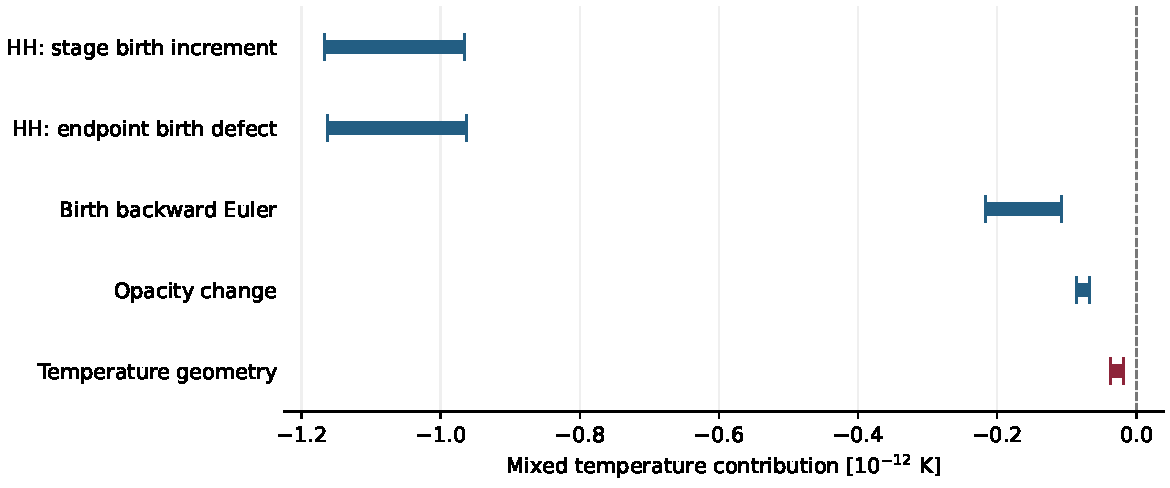
\includegraphics[width=0.96\linewidth]{figures/mixed_mechanism.pdf}
\caption{음의 혼합 응답을 결정하는 주요 항. HH와 광자 강제항은 같은
Full 역연산자와 온도 covector로 전달했다. 온도 geometry는 유한
quotient에서 별도로 더해지는 항이다. 광자 seven-sector의 일부 mixed
부호는 0을 포함하지만, 공통 광자 묶음은 음수로 포함된다.}
\end{figure}

두 HH 기울기 항은 각각 약 $10^{-12}\ {\rm K}$ 규모다. 명시적으로 분리한 다섯 HH
gradient 항을 원 우변에서 먼저 더한 후 공통 inverse로 전달하면
$[-2.329668009361,-1.928397581837]\times10^{-12}\ {\rm K}$다.
광자 일곱 항을 같은 방식으로 묶은 값은
$[-3.024678223968,-1.735793802686]\times10^{-13}\ {\rm K}$다.
나머지 기체와 endpoint 항의 합은
$[2.819648272515,11.40914739344]\times10^{-16}\ {\rm K}$로 작다.
온도 분수에서 추가되는 기하 항은
$[-3.666218766444,-1.794167181955]\times10^{-14}\ {\rm K}$다.

성분별 또는 묶음별 포함을 다시 합한 구간의 폭은 전체 우변을 한 번에
전달한 구간보다 조금 클 수 있다. 그 차이는 같은 참값에 대한 서로 다른
구간 표현에서 생긴다. 최종 채택값은 전체 상관 우변의 포함이다.
가장 큰 세 가지 성분별 폭은 stage HH gradient, endpoint HH gradient,
birth backward Euler이고 각각 약 $2.015\times10^{-13}$,
$1.994\times10^{-13}$, $1.091\times10^{-13}\ {\rm K}$다.
endpoint source Hessian 공간차 항의 폭은 약
$4.576\times10^{-16}\ {\rm K}$에 머문다.

\subsection{실행 기록과 교정}

주 application의 성공 실행은 wall $0.967359\ {\rm s}$,
CPU $0.930019\ {\rm s}$, peak RSS $43744\ {\rm KiB}$였다.
원 구간의 기여 묶음과 유한 사각형 귀결을 계산한 readout은
wall $0.114273\ {\rm s}$, CPU $0.070526\ {\rm s}$,
peak RSS $17568\ {\rm KiB}$였다. 두 결과는 별도 디렉터리에 동결했다.

첫 application은 guard를 숫자 인덱스로 읽어 \texttt{KeyError}가 났다.
원 guard의 이름은 \texttt{number}, \texttt{energy\_eV\_per\_H}였으므로
해당 필드 접근만 교정하여 다음 실행을 완료했다. 원 실패 source와
로그, 실행 자원 기록은 그대로 보존했다. 이는 자료 schema 접근의
구현 오류이며 원 물리 입력의 변경을 수반하지 않는다.

\subsection{실제 Wolfram과 xAct 검산}

Wolfram Language 15.0.1 Linux kernel에서 공식 xAct archive를
받아 SHA-256을 대조하고 xTensor 1.3.0을 실제로 불러왔다.
추상 지수 표준화에는 xPerm 1.2.4의 Wolfram Language group
algorithm을 사용했다. \texttt{\$xpermQ=False}는 tensor 정의와
\texttt{ToCanonical} 호출 전에 설정했다.

추상 지수 검산 7개는 mixed defect cancellation, bilinear 차,
균형 bilinear 차, stage Hessian 수축 차, Hessian mixed 대칭,
공통 adjoint, adjoint Hessian 대칭이며 모두 정확히 0이었다.
스칼라와 행렬 성분 14개도 모두 0이었다. 여기에 일반 $C^2$ mixed
chain rule, source mixed composition, HI Hessian 분모 차,
birth gradient 분모 차, mixed jet 곱과 역수, 유한 온도 quotient,
두 슬롯 비가환 remap의 seven-sector mixed 미분이 포함된다.
상징 연산 시간은 $1.216823\ {\rm s}$였다.

실행 서비스는 임의의 함수 기호 \texttt{HH18}, \texttt{B18}에 대해
\texttt{Symbol::undefined2} 진단을 출력했다. 두 기호는 일반 함수의
형식 미분을 비교하기 위해 의도적으로 미지정한 함수이며, 해당 도함수를
유지한 양변 차이가 0으로 단순화됐다. 원 진단과 실제 출력은 보존했다.
Wolfram context의 최초 내부 오류도 재시도 후 정상 응답한 환경 기록으로
구분한다. 35개 원 물리 슬롯의 수치 포함은 앞의 application이 담당한다.

\subsection{독립 검토의 판정}

별도 검토자는 후보 application 및 PHYS14 프로그램을 import하지 않고,
원 입력에 대한 자체 exact interval 산술과 Cramer determinant 방식의
선형 역 인증을 사용했다. 독립 arithmetic 22개 묶음이 모두 통과했다.
nilpotent polynomial 계수 합성으로 일곱 광자 항의
$7\times35\times4=980$개 성분을 각각 계산했으며,
모두 후보 포함 안에 들어갔다.

검토는 원 input identity, $U/V/W$와 parameter slot, Full birth의 2배
인수, 직접/상관 혼합 우변, 원 $C^2$ density bridge, stage mixed
increment, 유한 온도 분수, 공통 inverse의 세 기여 묶음을 포함한다.
mixed number/energy ledger는 두 guard를 유지한 잔차의 0 포함을
확인했다. 현재 수치의 음의 margin도 독립 유리수 계산과 일치한다.

독립 검사 첫 시도는 바깥쪽으로 저장된 decimal prior를 유리수
singleton으로 가정한 checker의 표현 오류를 발견했다. 실제 표현인
바깥쪽 구간 포함으로 판정식을 교정하여 다음 실행에서 22/22를
통과했다. 이 과정에서 생산 코드와 수치 결과는 바뀌지 않았다.
이론 정리 8개와 따름정리 4개는 이 범위에서 \texttt{PROMOTE\_SCOPED}로
채택한다. 남은 과학적 차단 사유는 없다. 실제 최종 해시와 채택은
\nolinkurl{review/INDEPENDENT_REVIEW.json},
\nolinkurl{review/DECISION.json}에 기록한다.


\section{문헌의 결과와 현재 구성의 관계}

SciSpace와 Exa로 2차 implicit sensitivity와 공통 관측량 adjoint를
검색하고 원문을 대조했다. Safiran--Lotz--Naumann의 정리 4.3은
parameterized nonlinear system의 2차 tangent를 원 state Jacobian과
Hessian 수축의 선형식으로 구성한다. 매개변수 seed를 서로 다른 두
좌표 방향으로 놓으면 이번 $J_FW_F=-\mathcal B(g_F;U_F,V_F)$와
일치한다. 이 implicit 관계는 원 $C^2$ 식에서 유도된다. 반복 Newton
알고리즘 자체를 두 번 AD하는 별도 구성의 미분 차수와 구별하여
적용했다.\cite{SafiranLotzNaumann2015}

Lewis의 정리 2.2와 식 (7)--(14)는 $C^2$ state equation과 관측량,
가역 state derivative 아래 tangent와 adjoint로 reduced Hessian을
구성한다. Pacaud 등의 2차 adjoint 구현도 Jacobian/transpose solve와
Hessian의 두 방향 수축을 결합한다. 이 구조는 하나의 Full inverse와
온도 covector로 현재 mixed forcing을 읽는 데 대응한다.
\cite{Lewis1997,PacaudEtAl2022}

Xue의 incremental state/adjoint 관계는 2차 implicit 검산의 현대적
비교 자료다. 현재의 전체 parameter-box 부호와 바깥쪽 오차 포함은
이 연구의 원 signed 자료 및 exact interval 연산에서 직접 얻었다.
\cite{Xue2025}

현재 구성은 표준 미분식을 WU088\_HH의 density bridge, 작은 결함,
같은 매개변수의 광자 chronology와 유한 온도에 연결한다.
원문 적용 위치와 접근 기록은
\nolinkurl{literature/LITERATURE_REVIEW_KO.md}에 있다.

\clearpage
\section{다음 연구와 재현 경로}

\subsection{현재 닫힌 항과 남은 순수 곡률}

현재 $F_\lambda,F_b,F_{\lambda b}$의 전역 포함은 확보했다.
축 위 실제 함수를 보존한 표현에서
\[
F=F(\lambda,0)+F(0,b)-F(0,0)+c_m\lambda b+R_m,
\]
\[
c_m=-2.393651191234\times10^{-12}\ {\rm K},\qquad
|R_m|\le2.748545551890\times10^{-13}\lambda b\ {\rm K}
\]
가 성립한다. $c_m$은 현재 바깥쪽 표시 구간의 중심이다.
이는 양 축의 비선형성을 보존하면서 교차항을 하나의 작은 계수와
검증된 잔차로 표현한 현재 결과다.

다음 노드는 \texttt{HH\_DEFECT\_PARAMETER\_CURVATURE}다.
두 남은 순수 곡률 $F_{\lambda\lambda},F_{bb}$를 원 $C^2$ 자료로
계산하여 축의 직선 보간까지 포함하는 전체 bilinear 모델의 오차를
구한다. $\theta\in\{\lambda,b\}$에 대해
\[
J_kg_{k,\theta\theta}
=-\{H_{k,gg}[g_{k,\theta},g_{k,\theta}]
+2H_{k,g\theta}g_{k,\theta}+H_{k,\theta\theta}\}
\]
가 출발식이다. Full과 첫 half에서는 고정 기체의 두 순수 parameter
partial이 0이고, carried 둘째 half에서는 이전 stage의 순수 incoming
jet를 함께 전달한다. 상세 식과 원자료 연결은
\nolinkurl{contracts/CURVATURE_CONTRACT.json}과
\nolinkurl{theory/NEXT_CURVATURE_PROPOSAL_KO.md}에 보존한다.

$M_{\lambda\lambda}\ge\sup|F_{\lambda\lambda}|$,
$M_{bb}\ge\sup|F_{bb}|$가 계산되면 네 실제 모서리를 잇는
$\mathcal L_{\rm bilin}F$에 대해
\begin{equation}
|F-\mathcal L_{\rm bilin}F|
\le\frac{M_{\lambda\lambda}}2\lambda(1-\lambda)
+\frac{M_{bb}}2b(1-b)
\label{eq:bilinear-remainder}
\end{equation}
를 얻는다. 각 축의 1차 보간 오차에 대한 Peano kernel 경계와
나머지 축 보간 연산자의 양성 가중치를 적용하면 이 부등식이 따른다.
현재 mixed 부호는 다음 계산의 확정 입력으로 재사용한다.
새 pure-curvature 수치 응답은 다음 단위의 실행 의무다.

그 실행에 필요한 첫 half의 선형 준비는 실제로 확인했다.
원 Jacobian 구간에서 $C_1=I$, $S_1=(1,1,1,27/2)$를 쓰면
exact rational 행 상계가
$q_1=0.0005395474227883633\ldots<0.0005396<1$이다.
독립 검토도 네 행 상계를 일치시켰다. 이는 새 pure 우변을 넣을
역 포함의 준비이며, 순수 곡률 응답의 수치 실행은 아직 하지 않았다.

\subsection{DAG와 현재 판정의 범위}

이번 DAG에서는 앞선 13개 HH 노드 값을 그대로 보존하고
\texttt{HH\_DEFECT\_MIXED\_RESPONSE}에 실제 계산과 독립 판정을 기록한다.
그 다음에 순수 곡률 노드를 추가한다. 원 global REI DAG 파일과
그 노드 상태는 기존 identity를 유지한다.
원 native/microscopic 경로의 과학적 조건을 보존하며 현재 작업에서
\texttt{heavy\_queue=[]}, \texttt{launch=false}를 유지한다.

\subsection{입력과 코드의 복원}

최종 연구 묶음에는 현재 core와 PHYS17의 고정된 최종 연구 archive가
들어 있다. 그 안의 PHYS16 묶음과 PHYS15 snapshot을 따라가면 실제
source, Hessian, carry와 원 전처리 자료를 복원할 수 있다.
각 부모는 자기 core 이름의 형제 디렉터리로 추출하며,
부모별 metadata는 별도 staging에 유지한다.
\nolinkurl{DEPENDENCIES.json}은 archive 크기와 SHA-256,
원 Git commit, 필요한 내부 경로를 결박한다.

\noindent\begin{minipage}{\linewidth}
복원한 작업 디렉터리에서 아래와 같이 새 출력 디렉터리를 지정한다.
성공한 기존 실행 디렉터리는 그대로 유지한다.
\begin{quote}\small
\ttfamily
python3 HH\_PHYS18\_THEORY\_20261013\_v1/src/\\
mixed\_response\_application.py \\
\quad --parent15 HH\_PHYS15\_THEORY\_20261012\_v1 \\
\quad --parent16 HH\_PHYS16\_THEORY\_20261013\_v1 \\
\quad --parent17 HH\_PHYS17\_THEORY\_20261013\_v1 \\
\quad --output PHYS18\_reproduce/results
\end{quote}
\end{minipage}\par
이 표시의 줄바꿈은 가독성을 위한 것이다. 복사 가능한 한 줄 명령은
\nolinkurl{checks/application/APPLICATION_KO.md}에 있다.
실제 Wolfram 검산은
\nolinkurl{checks/wolfram/mixed_response_checks.wl} 전체를
stateless evaluator에 주어 실행한다. 원 출력과 진단, archive/hash
확인은 같은 디렉터리에서 읽을 수 있다.

LaTeX source 묶음의 \texttt{latex/}에서 XeLaTeX, BibTeX, XeLaTeX 두 번
순서로 주 원고를 컴파일한다. 필요한 CJK font subset을 포함했다.
수치표와 그림은 동결된 exact 결과에서 생성한 것으로, PDF 재컴파일은
물리 source나 root 계산을 다시 실행하지 않는다.
정확한 명령과 실제 PDF 검증 기록은 \nolinkurl{report/BUILD_KO.md}와
\nolinkurl{report/qa/QA_RESULT.json}에 연결한다.

현재 판정, 완결한 R1--R10 단계, 원 실패와 교정, 다음 실행 의무는
\nolinkurl{state/RESEARCH_STATE.json}, \nolinkurl{HANDOFF_KO.md},
\nolinkurl{review/DECISION.json}에서 함께 추적한다.
최종 Git과 실제 Drive/Dropbox 저장 응답은 별도 delivery receipt에
기록하며, 과학 산출물의 identity와 저장 완료의 identity를 연결한다.

\bibliographystyle{unsrt}
\bibliography{references}
\end{document}
